\section{Results}
\begin{figure}[h]
\hspace{-2.8cm}
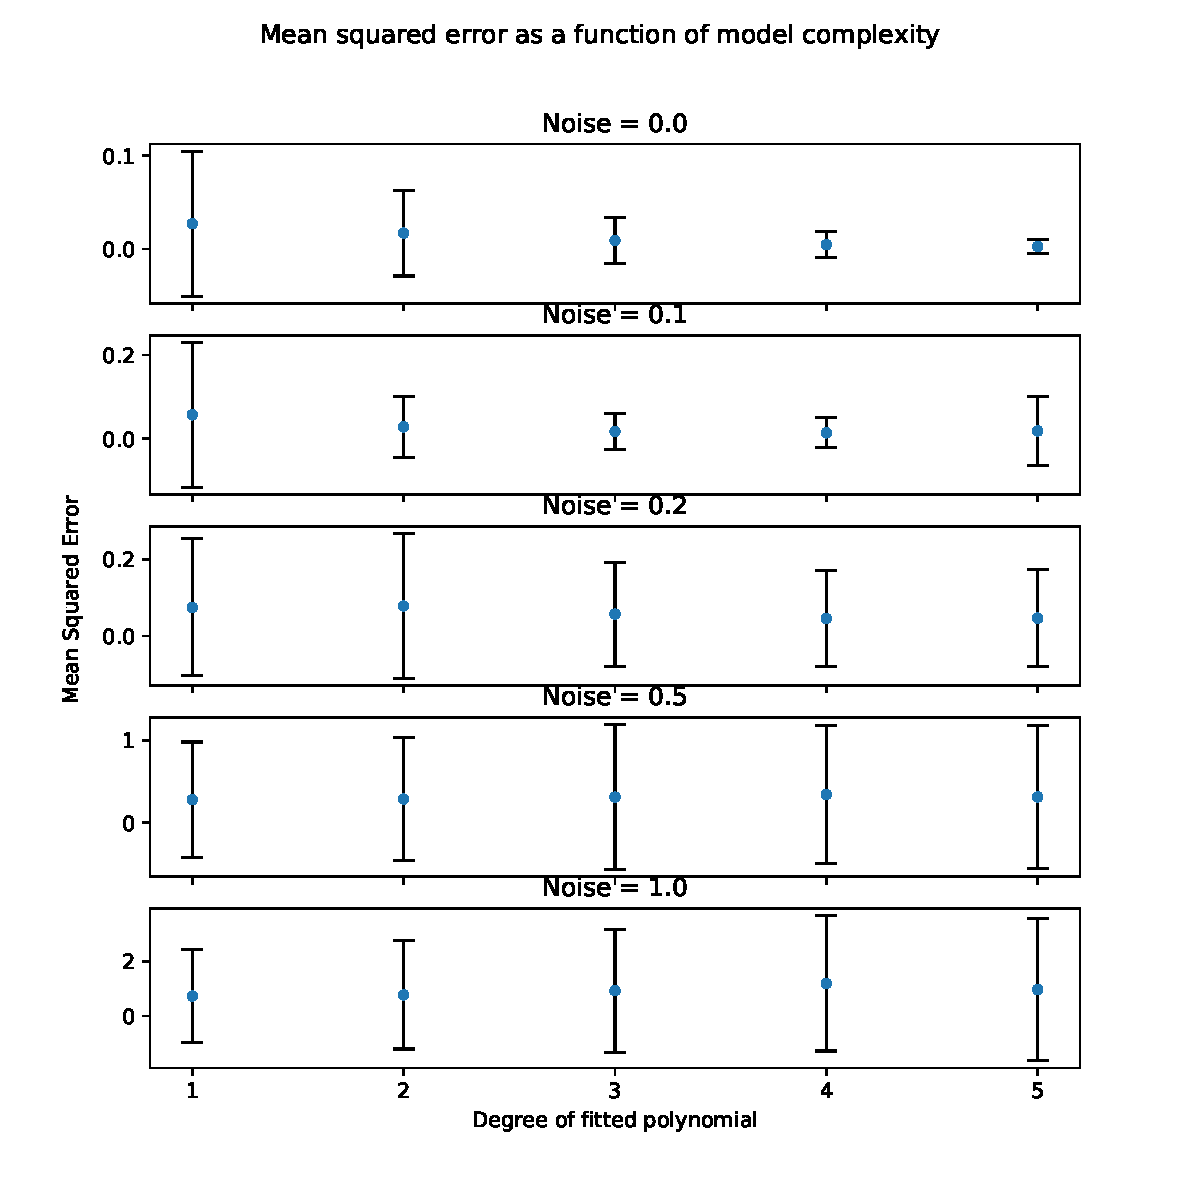
\includegraphics[width = \paperwidth]{figures/mse_vs_complexity_a.pdf}
\caption{Plot of Mean Squared Error as a function of model complexity (degree of the
	fitted polynomial). ols is ordinary least squares regression. The data used
	in this plots is the testing data generated by the Franke Function.}
\label{fig:mse-complexity-abc}
The plot in figure \ref{fig:mse-complexity-abc}
\end{figure}
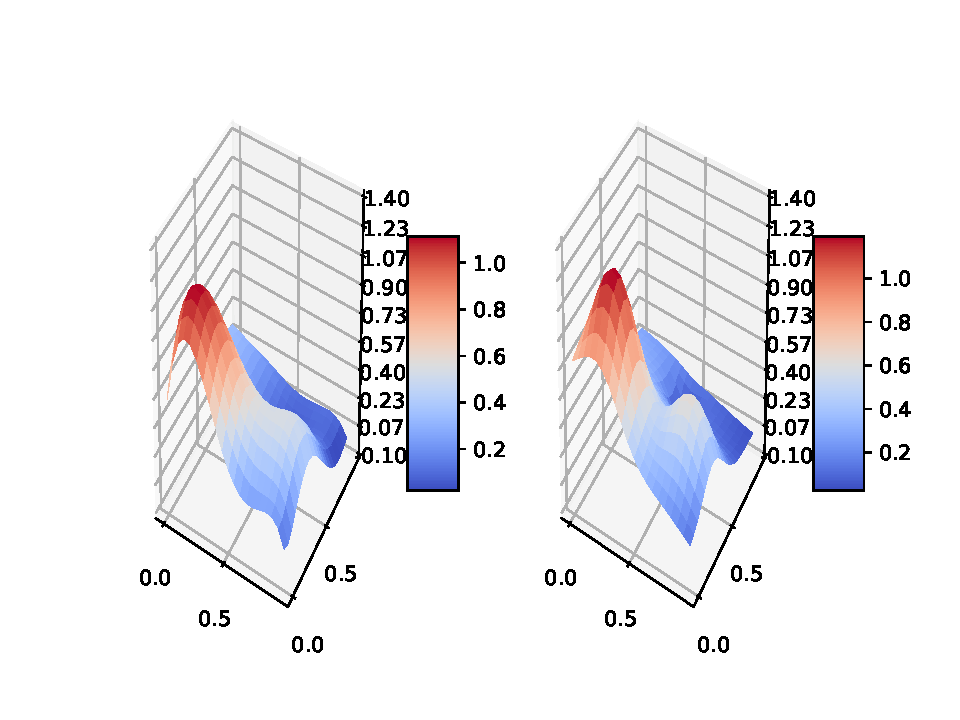
\includegraphics[width = \paperwidth]{figures/comparison_ols.pdf}
\caption{3D visualization of the polynomial fit with smallest mean squared error
	(left) and the original dataset generated by the Franke Function (right).
	The axes are unitless.}
\label{fig:mse-complexity-e}
\end{figure}
\begin{figure}[h]
\hspace{-2.8cm}
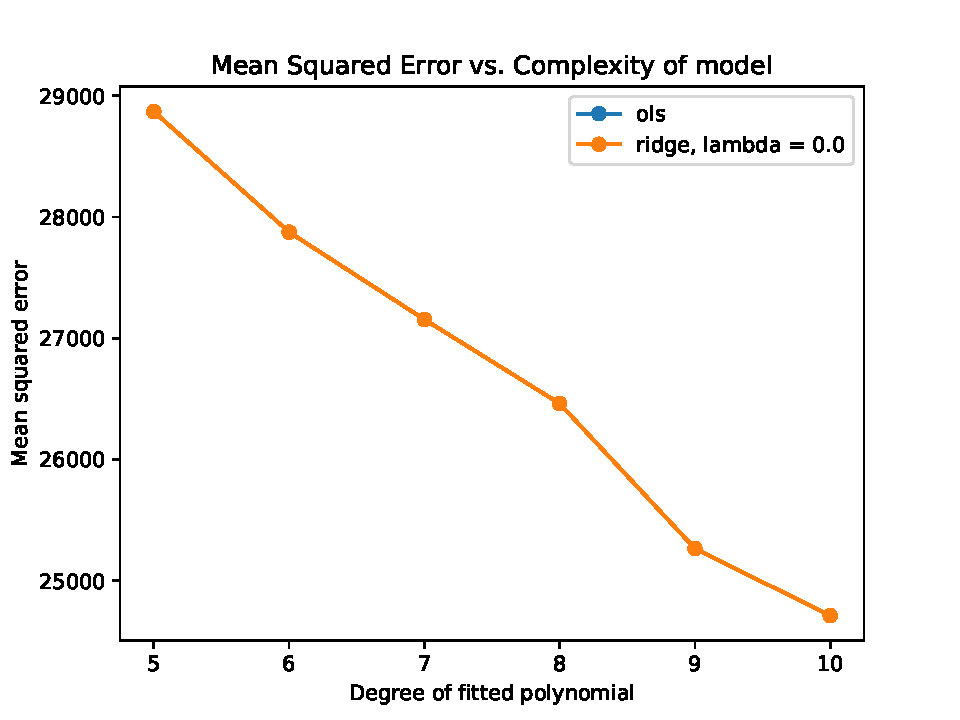
\includegraphics[width = \paperwidth]{figures/mse_vs_complexity_e_ols.pdf}
\caption{Plot of Mean Squared Error as a function of model complexity (degree of the
	fitted polynomial). ols is ordinary least squares regression.
	Regression was performed on real terrain data from a region in Norway.}
\label{fig:mse-complexity-e}
\end{figure}
\begin{figure}[h]
\hspace{-2.8cm}
\begin{figure}[h]
\hspace{-2.8cm}
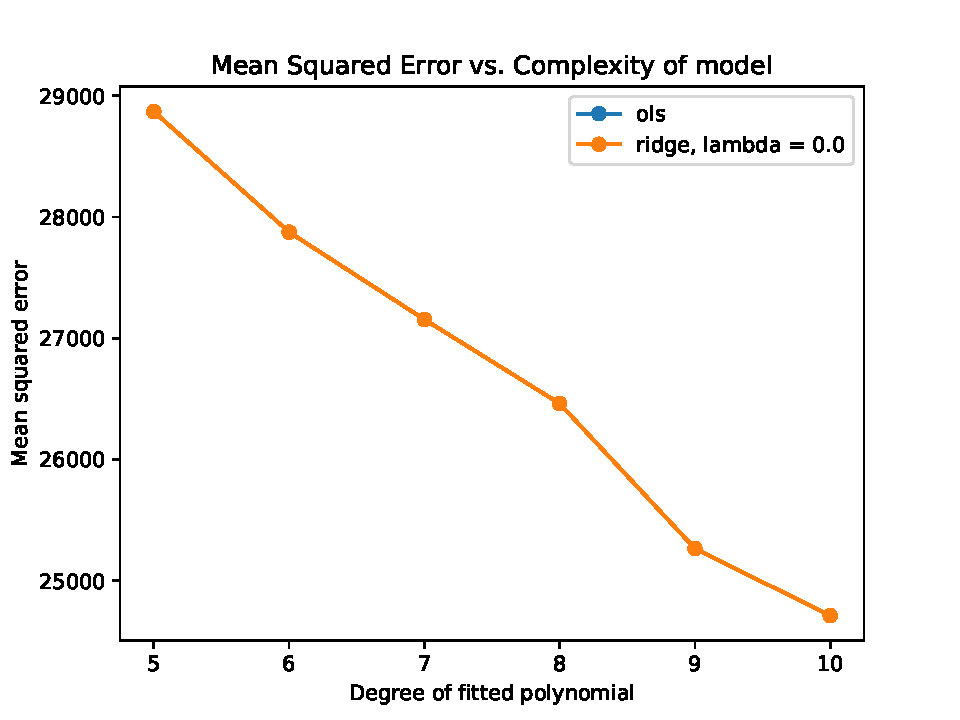
\includegraphics[width = \paperwidth]{figures/mse_vs_complexity_e_ols.pdf}
\caption{3D visualization of the polynomial fit with smallest mean squared error
	(left) and the original dataset from the terrain data (right).}
\label{fig:mse-complexity-e}
\end{figure}
